\documentclass[notes]{subfiles}
\externaldocument{lecture_11}

\begin{document}

\setcounter{section}{15}
\section{Lecture (3/31/25)}

\subsection{Laplace Transform}
The Laplace transorm is a special type of operator which does not use the same input variable as output variable. Instead of being able to consider the transform at each point of a function's domain, we consider the entire function as transformed, with no direct connection between the domains.

\begin{definition}[Integral Transform]
    Given a function $t \mapsto f(t)$, we define an \textit{integral transform} of $f$ as $s \mapsto F(s)$ such that
    \[
        F(s) = \int_a^b f(t)K(s, t)dt
    \]
    where $a, b$ are constant and $K$ is the \textit{kernel function} of the integral transform.
\end{definition}

\begin{example}
    The Fourier transform is an integral transform such that $a = -\infty$, $b = \infty$ and $K(s, t) = e^{2\pi i st}$.
\end{example}

\begin{definition}[Exponential Type]
    A univariate function $f$ is of \textit{exponential type} iff $|f(t)| \leq Me^{kt}$ where $M, k \in (0, \infty)$.
\end{definition}

\begin{example}[Exponential type functions]
    ~\par
    \begin{enumerate}[label = (\arabic*)]
        \item All polynomials are of exponential type.
        \item $\sin$ and $\cos$ are of exponential type.
        \item $t \mapsto ce^{at}$ for constants $c, a$
        \item Any bounded function is of exponential type.
    \end{enumerate}
\end{example}

\begin{example}[Non-exponential type functions]
    ~\par
    \begin{enumerate}[label = (\arabic*)]
        \item $t \mapsto \frac{1}{t}$ is not of exponential type since $\lim_{t \to 0^+} \frac{1}{t}$ is an infinite limit.
        \item $t \mapsto e^{t^2}$
        \item $\tan$
        \item $t \mapsto t^t$
    \end{enumerate}
\end{example}

\begin{definition}[Laplace Transform]
    Given a function $t \mapsto f(t)$ of exponential type, then the \textit{Laplace transform} $s \mapsto (\mathcal{L}f)(s)$ is the integral transform defined by
    \[
        (\mathcal{L}f)(s) = \int_0^\infty f(t)e^{-st}dt
    \]
    Note that we usually notate $F = \mathcal{L}f$, $G = \mathcal{L}g$, and so on.
\end{definition}

\begin{theorem}
    $\dom \mathcal{L}f = I$ where $I$ is an interval in $\mathbb{R}$.
\end{theorem}

We can view the Laplace transform as a continuous version of a generating function. With a generating function we get $a_n \mapsto \sum_{n = 0}^\infty a_n x^n$. In comparison, a Laplace transform gives us $f(t) \mapsto \int_0^\infty f(t)e^{-st}dt$.

\begin{exercise} \label{laplace_transform_base_case}
    Find the Laplace transform of $f$ as $f(t) = 1$.
\end{exercise}
\begin{solution}
    \begin{align*}
        F(s)
        &= \int_0^\infty f(t)e^{-st}dt
        = \lim_{b\to\infty} \int_0^b e^{-st}dt
        = \lim_{b\to\infty} \frac{-1}{s}e^{-st}\Big|_{t = 0}^{t = b}
        = -\frac{1}{s} \lim_{b\to\infty} (e^{-sb} - 1)
    \end{align*}
    Notice that if $s = 0$, then $F(s)$ does not exist due to the division by zero. Similarly if $s < 0$ then $\lim_{b\to\infty} (e^{-sb} - 1)$ is an infinite limit. Therefore $s > 0$ so
    \begin{align*}
        F(s)
        &= -\frac{1}{s} \lim_{b\to\infty} (e^{-sb} - 1)
        = -\frac{1}{s}(-1)
        = \frac{1}{s}
    \end{align*}
\end{solution}

This is a graph of the Laplace transform from \cref{laplace_transform_base_case}.

\begin{tikzpicture}[scale = 0.8]
    \begin{axis}[
        axis lines = middle,
        smooth,
        xlabel = $t$,
        ylabel = $f(t)$,
        xticklabel = \empty,
        yticklabel = \empty,
        grid = both,
        xmin = -1,
        xmax = 1,
        ymin = -1,
        ymax = 3
    ]
        \addplot[
            domain = -1:1,
            samples = 2,
            color = blue
        ] {1};
    \end{axis}
\end{tikzpicture}
\hspace{0.05\textwidth}
$\scalebox{2}{\ensuremath{\xrightarrow{\hspace{0.03\textwidth} \mathcal{L} \hspace{0.03\textwidth}}}}$
\hspace{0.05\textwidth}
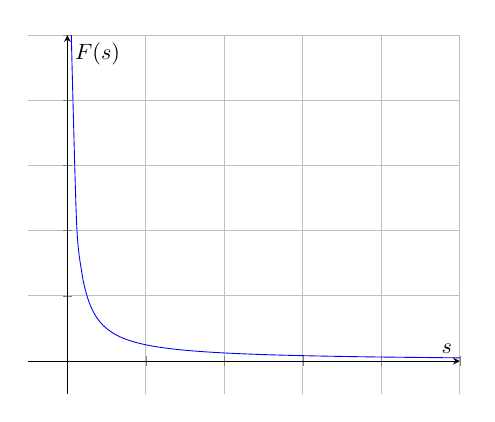
\begin{tikzpicture}[scale = 0.8]
    \begin{axis}[
        axis lines = middle,
        smooth,
        xlabel = $s$,
        ylabel = $F(s)$,
        xticklabel = \empty,
        yticklabel = \empty,
        grid = both,
        xmin = -1,
        xmax = 10,
        ymin = -1,
        ymax = 10
    ]
        \addplot[
            domain = 0.1:10,
            samples = 75,
            color = blue
        ] {1/x};
    \end{axis}
\end{tikzpicture}

\begin{exercise}
    Find the Laplace transform of $f$ as $f(t) = t$.
\end{exercise}
\begin{solution}
    \begin{align*}
        F(s)
        &= \int_0^\infty f(t)e^{-st}dt
        = \lim_{b\to\infty} \int_0^b te^{-st}dt
    \end{align*}
    Let $u = t \implies du = dt$ and $dv = e^{-st}dt \impliedby v = \frac{-1}{s}e^{-st}$
    \begin{align*}
        F(s)
        &= \lim_{b\to\infty} \int_0^b te^{-st}dt
        = \lim_{b\to\infty} \left( -\frac{t}{s}e^{-st}\Big|_{t = 0}^{t = b} + \frac{1}{s} \int_0^b e^{-st}dt \right)
        = \lim_{b\to\infty} \left( -\frac{t}{s}e^{-st} - \frac{1}{s^2} e^{-st} \right)\Bigg|_{t = 0}^{t = b} \\
        &= \lim_{b\to\infty} \left( -\frac{b}{s}e^{-sb} - \frac{1}{s^2}e^{-sb} - \frac{1}{s^2} \right)
    \end{align*}
    Like in \cref{laplace_transform_base_case} consider $s > 0$
    \begin{align*}
        F(s)
        &= \lim_{b\to\infty} \left( -\frac{b}{s}e^{-sb} - \frac{1}{s^2}e^{-sb} - \frac{1}{s^2} \right)
        = \lim_{b\to\infty} \left( -\frac{b}{se^{-sb}} - \frac{1}{s^2} \right)
        = \lim_{b\to\infty} \left( \frac{1}{s^2e^{-sb}} - \frac{1}{s^2} \right)
        = \frac{1}{s^2}
    \end{align*}
\end{solution}

Notice that $1 = t^0$ and $t = t^1$, this motivates the following lemma.

\begin{lemma}
    The Laplace transform of $f_n$ as $f_n(t) = t^n$ where $n \in \mathbb{Z}$ such that $n \geq 0$ is $F_n$ as $F_n(s) = \frac{n!}{s^{n + 1}}$.
\end{lemma}
\begin{proof}
    We already proved the base case of $n = 0$ in \cref{laplace_transform_base_case}. Therfore we consider our induction hypothesis $F_n(s) = \frac{n!}{s^{n + 1}}$   and want to show that $F_{n + 1}(s) = \frac{(n + 1)!}{s^{n + 2}}$.
    \begin{align*}
        F_{n + 1}(s)
        &= \int_0^\infty f_{n + 1}(t)e^{-st}dt
        = \lim_{b\to\infty} \int_0^b t^{n + 1}e^{-st}dt
    \end{align*}
    Let $u = t^{n + 1} \implies du = (n + 1)t^ndt$ and $dv = e^{-st}dt \impliedby v = \frac{-1}{s}e^{-st}$
    \begin{align*}
        F_{n + 1}(s)
        &= \lim_{b\to\infty} \left( -\frac{t^{n + 1}}{s}e^{-st}\Big|_{t = 0}^{t = b} + \frac{n + 1}{s}\int_0^b t^n e^{-st}dt \right) \\
        &= \lim_{b\to\infty} \left( -\frac{1}{s}b^{n + 1}e^{-sb} + \frac{n + 1}{s}\int_0^b t^n e^{-st}dt \right)
    \end{align*}
    Just like before, we only consider $s > 0$. Considering just $-\frac{1}{s}\lim_{b\to\infty} b^{n + 1}e^{-sb}$ we get
    \begin{align*}
        -\frac{1}{s}\lim_{b\to\infty} b^{n + 1}e^{-sb}
        &= -\frac{1}{s}\lim_{b\to\infty} e^{(n + 1)\ln b}e^{-sb}
        = -\frac{1}{s}\lim_{b\to\infty} e^{(n + 1)\ln b - sb}
    \end{align*}
    Notice that
    \begin{align*}
        \lim_{b\to\infty} ((n + 1)\ln b - sb)
        &= \lim_{b\to\infty} b\left((n + 1)\frac{\ln b}{b} - s\right)
        = \lim_{b\to\infty} b\left((n + 1)\frac{1}{b} - s\right) \\
        &= (n + 1) - sb
        = -\infty
    \end{align*}
    Therefore $-\frac{1}{s}\lim_{b\to\infty} e^{(n + 1)\ln b - sb} = 0$ so we get
    \begin{align*}
        F_{n + 1}(s)
        &= \lim_{b\to\infty} \left( -\frac{1}{s}b^{n + 1}e^{-sb} + \frac{n + 1}{s}\int_0^b t^n e^{-st}dt \right)
        = \frac{n + 1}{s}\lim_{b\to\infty} \int_0^b t^n e^{-st}dt \\
        &= \frac{n + 1}{s} \int_0^\infty f_n(s) e^{-st}dt
        = \frac{n + 1}{s} F_n(s)
        = \frac{n + 1}{s} \left( \frac{n!}{s^{n + 1}} \right)
        = \frac{(n + 1)!}{s^{n + 2}}
    \end{align*}
\end{proof}

\end{document}